
As discussed in \fref{sec:efficiency} and \ref{sec:quality}, there are
several measures for evaluating the quality of tests. This section
presents the results of these different metrics for the ECP software
before and after different parts of the case study.\\


\subsection{Test coverage}
    \label{sec:coverage_frameworks}

\subsubsection{Ruby test coverage}
There are multiple different ways of analyzing test coverage, and the
properties and conditions for each different kind of test coverage are
discoursed in \fref{sec:coverage}. However, we were unable to find any
test coverage tools for Ruby which analyzed anything else than statement
coverage, which is the weakest test coverage metric. Quite much effort
was spent on finding such tool, but without any success. Several
websites and Stack Overflow-answers indicate that no such tool exists
for Ruby at the time of this writing \cite{web:coverage_ruby19,
so:c1c2_coverage, so:c1_coverage, web:toolbox_code_metrics}. On one
hand, some of these sources are rather old and might be outdated, which
would indicate that such tool could have been created recently. On the
other hand would at least some of these sources probably been updated if
such tool became available.\\

We ended up using the
SimpleCov\footnote{\url{https://github.com/colszowka/simplecov}} tool
for Ruby test coverage metrics. At the time of this writing, it is the
most used Ruby tool for test coverage. It is also actively developed,
works with recent Ruby versions and RSpec versions, and produces pretty
and easy- to-read coverage reports in HTML (see
\fref{fig:simplecov_report}). \cite{web:toolbox_code_metrics}\\

\begin{figure}
\centering
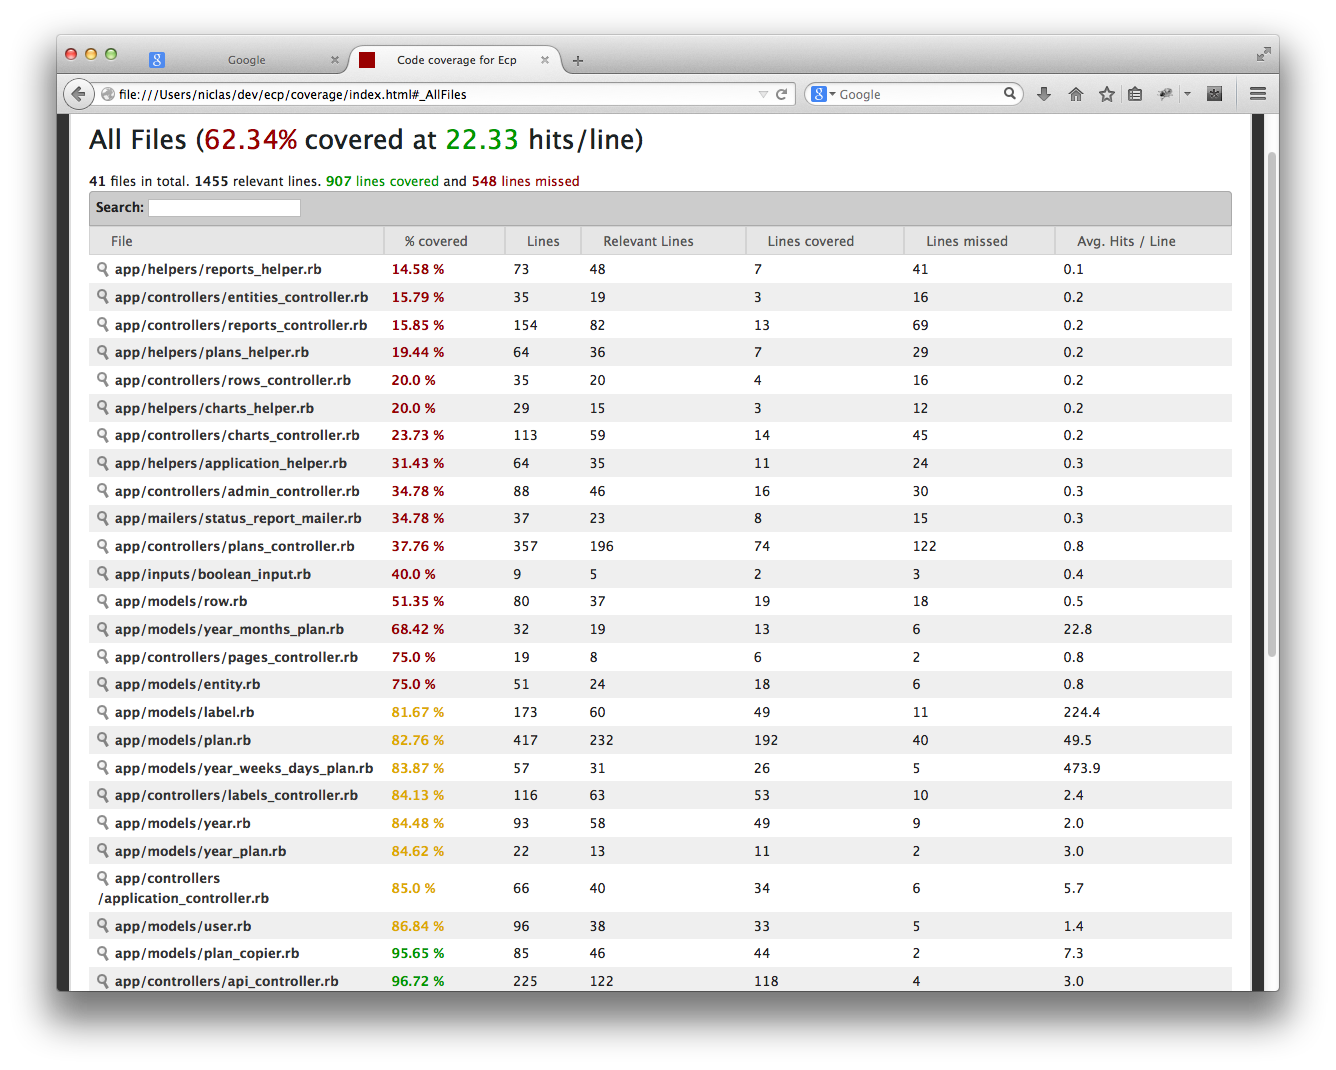
\includegraphics[width=0.8\textwidth]{results/choices/simplecov}
\caption{A test coverage report generated by SimpleCov.}
\label{fig:simplecov_report}
\end{figure}


\subsubsection{CoffeeScript test coverage}
For the client-side CoffeeScript, we used a plug-in for the Karma test
runner called karma-coverage\footnote{\url{https://github.com/karma-
runner/karma-coverage}}. This tool basically integrates Karma with
Ibrik\footnote{\url{https://github.com/Constellation/ibrik}}, which is a
tool developed by Yahoo! for measuring test coverage of CoffeeScript
code. We did initially have some problems with getting this tool to work
correctly, since Ibrik internally uses another CoffeeScript compiler;
CoffeeScriptRedux, than the compiler used when tests itself are run.
CoffeeScriptRedux is more strict and yielded syntax errors in some of
our files, which could be compiled correctly in the production code. The
latest available release of Ibrik (version 1.1.1) also had major issues
with certain constructs in CoffeeScript, which made the files impossible
to analyze. These issues were however fixed in the development version.
Ibrik was first released in December 2013, which may explain its
immaturity. Ibrik internally uses istanbul-js for the coverage
analysis and report generation.\\

The chosen solution worked very well after sorting out the issues.
Statement coverage as well as branch coverage is supported, and it
yields useful reports. As with SimpleCov, the coverage reports are
produced as an interactive HTML report (see \fref{fig:karma_report}).\\

\begin{figure}
\centering
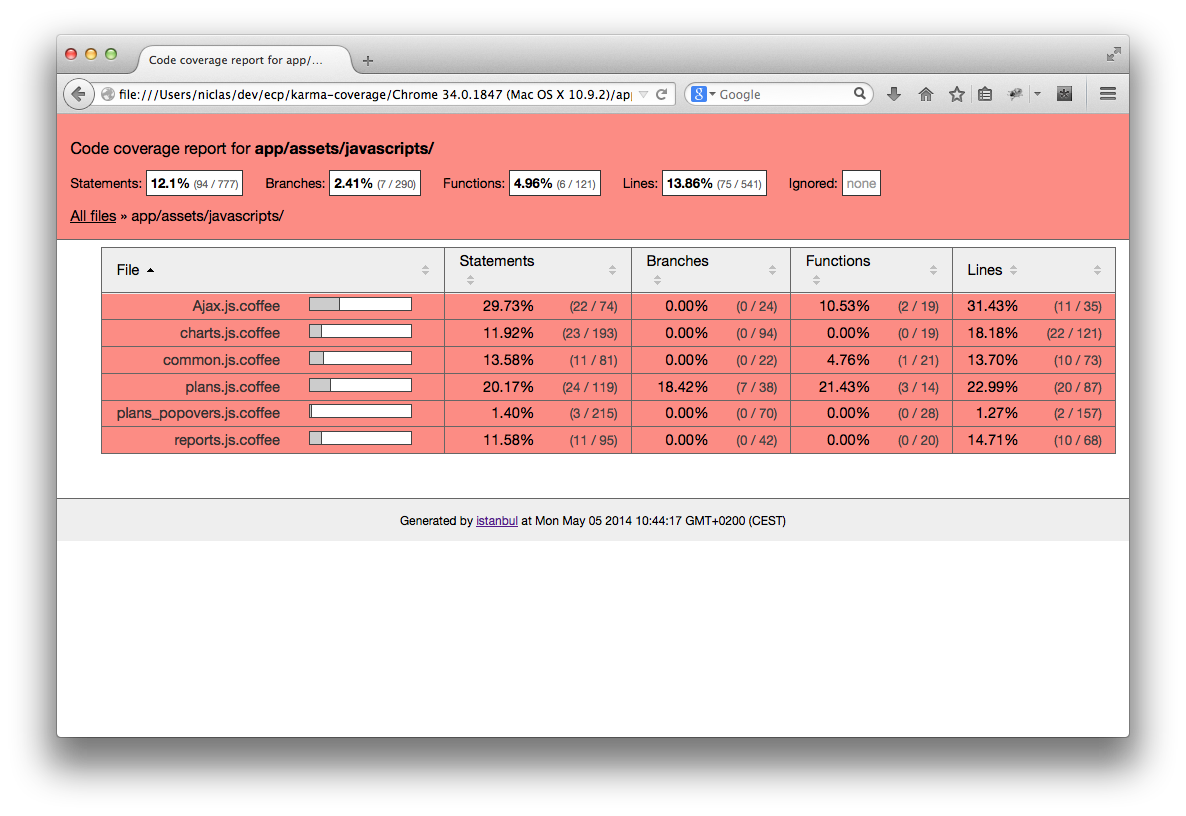
\includegraphics[width=0.8\textwidth]{results/choices/karma_coverage}
\caption{A test coverage report generated by istanbul-js using karma-coverage.}
\label{fig:karma_report}
\end{figure}


\subsubsection{Test coverage issues}

One issue with using test coverage in this particular project is the
fact that very few files were added. Most of the changes were made in
existing classes and files, either as new functions or as changes to
existing functions. Since the overall test coverage is measured per
file, it is impossible to get an exact measure of how well tested the
new and refactored code is, since old and completely untested code
lower the test coverage.\\

We have tried to mitigate this by looking at the coverage reports by
hand, and try to determine a subjective measure of how good the test
coverage is for new and refactored code. \Fref{fig:coverage_example}
shows an excerpt of a coverage report. In this case, our subjective
measure would say that the function |exports.getProduction()| is
completely untested. The function |exports.getLabelId()| is well tested
and has full statement- as well as branch coverage. The function
|exports.formatValues()| has full statement coverage, but non-optimal
branch coverage since the cases where |x| or |y| is not set are not
covered.\\

\begin{figure}
\centering
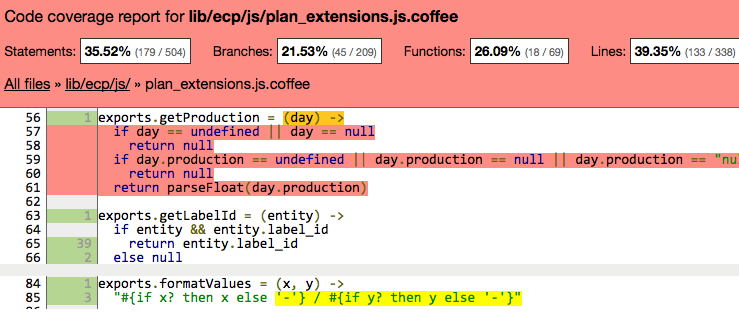
\includegraphics[width=0.8\textwidth]{results/choices/js_coverage}
\caption{An excerpt from a coverage report generated using karma-coverage
         which demonstrates three different types of tested functions.}
\label{fig:coverage_example}
\end{figure}


\subsection{Mutation testing}
    An alternative to draw conclusions from which paths of the code that is
run by a test, as done when using test coverage, is to draw conclusions
from what happens when we modify the code. The idea is that if the code
is incorrect, the test should fail. Thus, we can modify the code so it
becomes incorrect and then look at whether the test fails or not.\\

Mutation testing is done by creating several versions of the tested
code, where each version contains a slight modification. Each
such version containing a mutated version of the original source code is
called a \emph{mutant}. A mutant only differs at one location compared
to the original program, which means that each mutant should represent
exactly one bug.\cite{article:mutation, wiki:mutation}\\

\begin{lstlisting}[caption=Example of a piece of code before mutation,
                   label=lst:mutation_before, float=t]
    def odd?(x, y)
        return (x % 2) && (y % 2)
    end
\end{lstlisting}


\begin{lstlisting}[caption=Mutated versions of \ref{lst:mutation_before},
                   label=lst:mutation_after, float=t]
    def odd?(x, y)
        return (x % 2) && (x % 2)
    end

    def odd?(x, y)
        return (x % 2) || (y % 2)
    end

    def odd?(x, y)
        return (x % 2) && (0 % 2)
    end

    def odd?(x, y)
        return (x % 2)
    end
\end{lstlisting}

There are numerous ways of creating mutations to be used in mutants. One
could for example delete a method call or a variable, exchange an
operator for another, negate an if-statement, replace a variable with
zero or null-values, or something else. Code listing
\ref{lst:mutation_before} shows an example of a function which should
return true if both arguments are odd. Several mutated versions of this
example is shown in code listing \ref{lst:mutation_after}. The goal of
each mutation is to introduce a modification similar to a bug introduced
by a programmer.\cite{article:mutation}\\

All tests which we want to evaluate are run for the original program as
well as for each mutant. If the test results differ, the mutant is
considered to be \emph{killed}, which means that the test suite has
discovered the bug. Some mutants may however have a change that does not
change the functionality of the program. An example of this can be seen
in \ref{lst:mutation_eq}, where two variables are equal and therefore
not affected by replacing one of them with the other. This is called
an \emph{equivalent mutant}. The goal is to kill all mutants which is
not equivalent mutants.\cite{article:mutation, wiki:mutation}\\

\citet{article:mutation} presents the results of an experiment where
mutation testing was used in a web application with an automatically
generated test suite. Over 4500 mutants was generated, with a test suite
of 38 test cases. Running each test case for each mutant would require
over 170000 test runs. A large part of the program was therefore
discarded and the evaluation was focused on a specific part of the
software, which left 441 mutants. 223 of these was killed, 216 was
equivalent and 2 was not killed.\\

The article by \citeauthor{article:mutation} exemplifies two challenges
with mutation testing; a large amount of possible mutants, and a
possibly large amount of equivalent mutants. In order for mutant testing
to be efficient, the scope of testing must be narrow enough, the test
suite must be fast enough, and equivalent mutants must be possible to
detect or not be generated at all. \citeauthor{article:mutation} uses
manual evaluation to detect equivalent mutants, which is probably
impracticable in practice. \citet{article:eq_mutant} presents an
overview of multiple ways of dealing with equivalent mutants, but
concludes that even though some approaches looks promising, there is
still much work to be done in this field.\\

\begin{lstlisting}[caption=Example of a program with an equivalent mutant,
                   label=lst:mutation_eq, float=t]
    def some_function(x)
        i = 0
        while i != 2 do
            x += 1
        end
        return x
    end

    def equivalent_mutant(x)
        i = 0
        while i < 2 do
            x += 1
        end
        return x
    end
\end{lstlisting}


\subsection{Execution time}
    
\subsection{Development of test execution time during the project}

As seen in \fref{sec:results_time}, the execution time of the RSpec
integration- and unit tests has decreased for every part of the case
study, even though the number of tests has increased. On average, each
test is more than twice as fast after the second part compared to before
the case study.\\

The major reason for the increase of speed comes from the refactoring of
old tests, initiated in the first part of the case study. Some old tests
were also refactored during the second part, which explains the decrease
in test execution time between the first and the second part of the case
study. One reason for the drop in average execution time after the
second part was also the fact that a few more unit tests was written,
compared to before.\\

The single most important factor for speeding up tests when refactoring
the old tests was to reduce the construction of database objects. Before
the case study, all test data for all tests was created before every
test, since the database needs to be cleaned between each test in order
for one test not to affect other tests. By using factory objects, I
could instead create only the objects needed for each specific test,
instead of creating a huge amount of data that is not even used. RSpec
also caches factory objects between tests that use the same objects,
which gives some additional speed gain.\\


\subsection{Execution time for different test types}

In \fref{sec:theory_levels}, we discussed different levels of testing,
and how this affects the amount of executed code and the test execution
time. \Fref{tab:jasmine_times} shows that our isolated Jasmine unit
tests runs at a rate of over 700 tests per second, while our system-level
browser tests in \fref{tab:rspec_browser_times} runs at a rate of
less than 0.3 tests per second. I would therefore say that the principle
of writing many isolated unit tests and a few system tests seems
very reasonable unless we choose to discard the execution time
completely.\\

One other interesting thing is the large difference between the Cucumber
browser tests and the RSpec browser tests. Even though both types of
tests are in the category of system tests, RSpec browser tests are more
than four times faster than the Cucumber tests. One reason for this
might be the size of the test. As seen in \fref{tab:browser_coverage},
the Cucumber tests cover more code than the RSpec browser tests, and
therefore take longer time to execute.\\

Another reason for the large difference in execution time might be that
some Cucumber tests are redundant. For example, the Cucumber test suite
tests login functionality multiple times, while the RSpec browser test
suite only tests this functionality once. This is because a logged-in
user is required in order to execute most tests, and the Cucumber tests
does this by entering credentials into the login form for each test. The
RSpec test suite instead uses a test helper to log in the user before
each test starts, except for when testing the login form itself. Yet
another reason for the execution time difference might be the overhead
of parsing the ubiquitous language used by Cucumber.\\


\subsection{Importance of a fast test suite}

One may argue that there is no reason to have a fast test suite, and one
may also argue that a fast test suite is very important. I think the
importance of tests being fast depends on the mindset on the people
writing them, how often the tests are run and in which way. I will
discuss some of my own experiences on this topic.\\

Having a super-fast unit test suite such as our Jasmine tests is really
nice when using TDD methodology, since it feels like the whole test
suite is completed in the same moment a file is saved. However, using
RSpec integration tests, which runs in about 150 ms, also works
fine when using TDD-methodology as long as we only run tests for the
affected module. Running the whole integration test suite continuously
takes too much time, though.\\

For the RSpec tests, the startup time before tests actually are run is
considerably long, since Rails and related components are very large and
takes some time to load. It would be possible to separate parts of the
test suite from Rails and associated frameworks as mentioned in
\fref{sec:theory_time}, but I refrained from doing this since I
considered it to affect the code structure in a bad way. Using tools
like Zeus\footnote{\url{https://github.com/burke/zeus/}} can work around
this problem, but I was unable to evaluate this tool due to
incompatibilities with my Ruby version.\\

For browser tests, I believe that the most important thing is the ability to
run these in some reasonable time. In this particular case, I believe
that the RSpec browser test suite fast enough to be run before each
deploy without annoyance, while the Cucumber suite barely fulfills the
criterion of being run within \quotes{reasonable time}. A good approach
would be to eventually re-factor the Cucumber test suite into unit-,
integration- and RSpec browser tests. Running browser tests on a
separate testing server instead of locally is another alternative.\\


